\documentclass{article}
% \usepackage{handout}
\usepackage{preamble}
\usepackage{graphicx} % Required for inserting images
\usepackage{amsmath}
\usepackage{physics,mlmodern}

\newcommand{\ddelta}{$\delta^{3}(\vb{r})$}
\title{Physics}
\author{Sabarno Saha}
\date{February 2023}

\begin{document}

\maketitle
\newpage
\tableofcontents
\newpage
\section{Magnus effect }
This article aims to further strengthen the understanding of the Magnus effect by finding a direct correlation between the Bernoulli Fluid Equation and the Magnus force. The Magnus force is force that affects "rapidly" spinning bodies in the direction perpendicular to their movement. Now here comes the construction from the Bernoulli equation.
\subsection{Analytical approach}
Suppose a cylinder moves forward so the "faster" moving surface "pulls" the air up and in turn gets pulled down due to newton's Third law.
\subsection{Scenario}
There is a cylinder moving in space in the direction $+\hat{x}$. Now the cylinder is given an angular velocity $\omega$ which points in the $+\hat{k}$ direction.Therefore the ball spins counter clockwise.
\subsection{Derivation}
We start of with the Bernoulli equation from fluid dynamics.
In this case the terms are as follows: $P_0$ refers to the ambient pressure, $\frac{1}{2}\rho v^2$ refers to the dynamic pressure, the last term can be ignored here as the cylinder used for measuring the Magnus effect can be taken to be arbitrarily small causing the height difference to be negligible.
\begin{equation}
    P_0 + \frac{1}{2}\rho v^2 +\rho_0 gh = \kappa \\
\end{equation}
The ambient pressure change essentially gives rise to the change in the pressure between the high and low spinning sides of the cylinder causing the Magnus effect. So here the term $v$ represents the fluid velocity. here the fluid velocity is the velocity is the velocity of a small elemental part of the fluid. Now let us define two pressures of the cylinder in question. Let the top pressure be denoted by $P_t$ and the bottom surface pressure be denoted by $P_b$. Now let the ball move from left to right in this question (suppose$\hat{x}$ with velocity u).
\begin{align*}
    P_t &= \kappa - \frac{1}{2}\rho(v-r\omega)^2\\
    P_b &= \kappa - \frac{1}{2}\rho(v+r\omega)^2\\
\end{align*}
To understand the above equations let us enter the COM frame of the object(only translation frame not the spinning frame). This essentially allows us to set the velocity of air in direction $-\hat{x}$. So now we need the fluid velocity at the top of the cylinder and the bottom of the cylinder. The fluid velocity is the relative velocity of the air with respect to the top surface of the cylinder. At the top part of the cylinder we have $v_r = v-r\omega$ as the ball is spinning in direction opposite to the velocity at that point. Similarly the expression for the bottom velocity can also be defined.
\begin{align*}
    \Delta P &= |-\frac{1}{2}\rho(v-r\omega)^2 +\frac{1}{2}\rho(v+r\omega)^2|\\
    \Delta P &= |2\rho v r \omega|
\end{align*}
This $\Delta P$ is in the net direction downward i.e. in the direction $\omega \times v$. This net pressure change gives us an important fact that there will be a net force downward causing the ball to 'curl'.
\subsection{Conclusion}
So essentially we can define the Magnus force as:
\begin{align*}
\fbox{$\vb{F_{magnus}} = S(v)\vb*{\omega\times v}$}
\end{align*}
Now there is a lack of published formula on the Magnus Effect because there are multiple formulae that yield different results. We can assume irrotational flow which gives us the above definition of the Magnus effect. But , without assuming the irrotationality of the flow we can assume that the liquid is being pulled away due to the centrifugal force and thus needs an added pressure gradient to balance out the centrifugal force experienced by the liquid. Further on that later.
\subsection{Post Notes}
The defined formula for the Magnus effect has not been published yet as the defined formulae come out to be different for different models of the fluid flow taken and the assumptions made in the liquid's movement. The general formula written above is True but the formula for $S(v)$ is not defined properly.
\subsection{Extra Reading}
\begin{enumerate}
    \item Irrotational Flow in Fluids(Richard Fitzpatrick)
    \item Potential Flow around a cylinder
    \item David Tong (Fluid Dynamics)
    \item Flow past a circular cylinder
\end{enumerate}
\section{Alternate form Of Griffiths 3.36 TBC}
\subsection{Question}
\begin{question}
Show that the electric field of a (perfect) dipole can be
written in the coordinate-free form:\\ 
\fbox {$E_{dip(r)} = \frac{1}{4\pi\epsilon_0}\frac{1}{r^3}3[(\va{p}\cdot\vu{r})\vu{r} -\va{p}]$}
\end{question}

\subsection{Derivation}
This formula is dependent on the fact that the dipole is oriented towards the $\vu{z}$ direction. The one we derive that assumes nothing other than the fact that the dipole moment does not depend on the azimuthal dependence $\phi$. \\ \\ \\
\begin{align*}
    \va{E} = -\grad V\\
    V = \frac{1}{4 \pi \epsilon_0} \iiint_\mathbf{V}r'\rho(r')d\tau\\
    \vb{p} = 
\end{align*}

\section{Mpemba Effect}
\subsection{Introduction}
The Mpemba effect is the name given to the observation that a liquid (typically water) which is initially hot can freeze faster than the same liquid which begins cold, under otherwise similar conditions. There is disagreement about its theoretical basis and the parameters required to produce the effect. This is a quite confusing effect with very varying theoretical explanations. This was first shown by Aristotle but was named after an african student named Erasto Mpemba whose demonstration in a class of the said effect attained widespread attention. A more precise statement is stated as follows:
\subsection{Statement}
\begin{example*}
    There exists a set of initial parameters, and a pair of temperatures, such that given two bodies of water identical in these parameters, and differing only in initial uniform temperatures, the hot one will freeze sooner.\\
\includegraphics[width = 4.5in]{Mpemba_Effect_temperatures_plot.png}
\end{example*}
\subsection{Proof}
honestly have no fucking idea how this works. There are multiple explanations of which i understand none. Refer to the wikipaedia page for further jargonic explanations.
\newpage
\section{Euler's Laws of Motion}
\subsection{Introduction}
The Eulerian Laws of motion states the newton's laws only for the case of rigid bodies by changing newton's laws to accommodate for the fact that the newton's laws only hold for a system of discrete particles. Euler then formulated the Newton's Laws for rigid bodies.
\subsection{Euler's First Law}
\subsubsection{Statement}
\begin{example*}
    Euler's First Law states that the rate of change of linear momentum of a rigid-body $\vb{p}$ is equal to the resultant of all the external forces acting on the body $\vb{F_{ext}}$.
\begin{align*}
    \vb{F_{ext}} = \frac{d\vb{p}}{dt}
\end{align*}
\end{example*}
\subsubsection{Proof}
This is a direct result of Newton's Third Law. This states that "When one body exerts a force on a second body, the second body simultaneously exerts a force equal in magnitude and opposite in direction on the first body."

Also from Newton's Second Law we get that total force is equal to the rate of change of linear momentum.
\begin{align*}
    \vb{F_{total}} &= \vb{F_{int}} + \vb{F_{ext}}\\
\end{align*}
\text{We can mathematically show that the net internal Force wrt to the centre of mass will be 0.}
\\
Now we can prove the following for a system of n-particles and extend it later for continuous objects.
\begin{align*}
    \vb{F_{total}} &= \vb{F_{int}} + \vb{F_{ext}}\\
    \vb{f_{ij}} &= -\vb{f_{ji}}\text{     }\forall i,j\leq n,i\neq j \\
    \implies \sum_{i\neq j} \sum_j \vb{f_{ij}} &=0\\
    \implies \vb{F_{int}} &=\sum_{i\neq j} \sum_j \vb{f_{ij}}\\
    & = 0\\
    \vb{F_{total}} &= \frac{d\vb{p}}{dt} \text{          From N2L}\\
    \vb{F_{total}} &= \vb{F_{int}} + \vb{F_{ext}}\\
    \text{But    } \vb{F_{int}} &= 0\\
    \implies \vb{F_{total}} &= \vb{F_{ext}}\\
    \implies \vb{F_{ext}} &= \frac{d\vb{p}}{dt}
\end{align*}
This proves Euler's First Law by invoking Newton's Laws. If we tend n to $\infty$ and the partitions are done tending to 0. We can replace the $\sum$ with an $\int dx$ essentially getting to the law for continuous objects.\\
\begin{align*}
    \vb{F_{ext}} &= \frac{d\vb{P}}{dt}
\end{align*}
\subsection{Euler's Second Law}
\subsubsection{Statement}
\begin{example*}
    Euler's second law states that the rate of change of angular momentum L about a point that is fixed in an inertial reference frame (often the center of mass of the body), is equal to the sum of the external moments of force (torques) acting on that body M about that point:\\
\begin{align*}
    \vb{M} &= \frac{d\vb{L}}{dt}
\end{align*}
    which can also be restated as the following in a different inertial frame. For rigid bodies translating and rotating in only two dimensions, this can be expressed as:\\
\begin{align*}
    \vb{M} &= m(\vb{r_m}\times \vb{a_m}) + \vb{I}\vb*{\alpha}
\end{align*}
\textbf{\begin{enumerate}
    \item[\vb{r_{m}}] : the position vector of the center of mass of the body with respect to the point about which moments are summed,
    \item[\vb{a_m}] : the linear acceleration of the center of mass of the body,
    \item[\vb{m}] : mass of the body
    \item[\vb{I}] : moment of inertia of the body w.r.t the centre of mass of the body
\end{enumerate}
\end{example*}
}
\subsubsection{Proof}
We now try to prove the law using a system of n-particles which we will again extend to continuous objects by assuming there to be infinite particles made up by very small chunks of the continuous body.\\
\begin{align*}
    \va{L} &= \va{r}\cp\va{p}\\
    \dv{\va{L}}{t} &=\dv{\va{r}}{t}\cp\va{p} + \va{r}\cp\dv{\va{p}}{t}\\
    &= \va{r}\cp\dv{\va{p}}{t}\\
    &= \va{r}\cp\va{F}\\
    &= \va{M}\\
\end{align*}
Thus we have proved the first part of Euler's Second Law. Now we come to the second part of the Law.
\begin{align*}
    \Dot{\omega} &= \vb*{\alpha}\\
    \va{L} &= m(\va{r}\cp\va{v})\\
    \text{For a system }& \text{of n-particles we have}\\
    \va{L} &= \sum m_i(\va{r_i}\cp\va{v_i})\\
    \text{In COM frame}&\\
    \va{r_i} &= \va{d_i } + \va{R}\\
    \text{where d is the distance}&\text{ of the particle from the centre of mass}\\
    \text{where R is the distance}&\text{ of the centre of mass from the original reference point}\\
    \va{L} &= \sum m_i((\va{d_i }+\va{R})\cp(\Dot{\va{d_i}}+\va{\Dot{R}}))\\
    \va{L} &= \sum m_i(\va{d_i }\cp\Dot{\va{d_i}}) + \sum m_i(\va{d_i }\cp\Dot{\va{R}})+\sum m_i(\Dot{\va{d_i }}\cp\va{R}) + \sum m_i(\va{R} \cp\Dot{\va{R}})\\
\end{align*}
The $\va{d_i}$ and  $\Dot{\va{d_i }}$ only terms get summed over to 0. because of the fact that the terms are calculated w.r.t. to the COM frame. As a result the weighted sum comes out to be 0.
\begin{align*}
     \va{L} &= \sum m_i(\va{d_i }\cp\Dot{\va{d_i}}) + \sum m_i(\va{d_i }\cp\Dot{\va{R}})+\sum m_i(\Dot{\va{d_i }}\cp\va{R}) + \sum m_i(\va{R} \cp\Dot{\va{R}})\\
      \va{L} &= \sum m_i(\va{d_i }\cp\Dot{\va{d_i}}) +\sum m_i(\va{R} \cp\Dot{\va{R}})\\
      \va{L} &= \sum m_i(\va{d_i^2}\omega) +\sum m_i(\va{r_{cm}} \cp\va{v_{cm}})\\
      \va{L} &= I\omega +\sum m_i(\va{r_{cm}} \cp\va{v_{cm}})
\end{align*}
Now using the first part of Euler's Second Law we take the derivative of $\va{L}$.
\begin{align*}
    \dv{\va{L}}{t} &= I\dv{\omega}{t} + \sum m_i(\va{r_{cm}} \cp\dv{\va{v_{cm}}}{t})\\
    \va{M} &= I\va*{\alpha} + \vb{m}(\va{r_{cm}} \cp\va{a_{cm}})\\
\end{align*}
This proves the second part of the law.


\newpage
\section{Euler's Equations of motion}
\subsection{Equations}
\begin{example*}
In classical mechanics, Euler's rotation equations are a vectorial quasilinear first-order ordinary differential equation describing the rotation of a rigid body, using a rotating reference frame with angular velocity ω whose axes are fixed to the body. Their general vector form is 
\begin{align*}
\vb{I}\dot{\va*{\omega}} + \va*{\omega} \times (\vb{I}\va*{\omega}) &= \va*{\tau} \
\end{align*}
In this equation, $\boldsymbol{\omega}$ is the angular velocity vector, $\mathbf{I}$ is the inertia tensor, and $\boldsymbol{\tau}$ is the external torque vector. The notation $\boldsymbol{\omega} \times \mathbf{I}\boldsymbol{\omega}$ represents the vector cross product of $\boldsymbol{\omega}$ with the matrix product of $\mathbf{I}$ and $\boldsymbol{\omega}$. The dot above $\boldsymbol{\omega}$ represents the time derivative of the vector $\boldsymbol{\omega}$.\\
\\
Now if we replace $\vb{I}$ tensor to not have off diagonal elements\\
\begin{align*}
\mathbf{I} =
\begin{pmatrix}
I_1 & 0 & 0 \\
0 & I_2 & 0 \\
0 & 0 & I_3 \\
\end{pmatrix}
\end{align*}
Then we can individually evaluate each element to arrive at the expressions: \\
\begin{align*}
\frac{d}{dt}\left(I_1\omega_1\right) - (I_2 - I_3)\omega_2\omega_3 &= \tau_1 \\
\frac{d}{dt}\left(I_2\omega_2\right) - (I_3 - I_1)\omega_3\omega_1 &= \tau_2 \\
\frac{d}{dt}\left(I_3\omega_3\right) - (I_1 - I_2)\omega_1\omega_2 &= \tau_3 \\
\end{align*}
In this equation, $I_1, I_2,$ and $I_3$ are the moments of inertia about the principal axes of a rigid body, $\omega_1, \omega_2,$ and $\omega_3$ are the angular velocities about those axes, and $\tau_1, \tau_2,$ and $\tau_3$ are the external torques acting on the body about those axes.
\end{example*}
\subsection{Proof}
Using Euler's Laws of Motion in an inertial frame of reference, we have,
\begin{align*}
    \dv{\vb{L_{in}}}{t} &= {\tau _{in}}\\
    \vb{L_{in}} &= \vb{I_{in}}\va*{\omega}\\
\end{align*}
When we change the frame of motion to a rotational frame of reference, we get:
\begin{align*}
    \dv{\vb{L}}{t} + \va*{\omega} \times \vb{L} &= {\tau} \\
    \implies \vb{I}\dot{\va*{\omega}} + \va*{\omega} \times \vb{I}\va*{\omega} &= {\tau}
\end{align*}
Thus we have derived Euler's equations of motion. Explicitly evaluating a component might give us the component form given to us in the second part of the derivation. This also can be written generally in einstein summation form using the ij components and representing the cross product using the Levi-Civita Tensor.
\begin{align}
    \vb{I_{ik}}\dot{\omega_{kj}} + \epsilon_{ijk}\omega \times \vb{I}\va*{\omega} &= {\tau_i}
\end{align}
Explicitly solving each of the components will result  to the solutions that are present in the second part of the compoennt part of the Euler's equations.
\newpage
\section{Intermediate axis Theorem/Tennis racket theorem}
\subsection{Introduction}
The tennis racket theorem or intermediate axis theorem is a result in classical mechanics describing the movement of a rigid body with three distinct principal moments of inertia. It is also dubbed the Dzhanibekov effect, after Soviet cosmonaut Vladimir Dzhanibekov who noticed one of the theorem's logical consequences while in space in 1985, although the effect was already known for at least 150 years before that and was included in a book by Louis Poinsot in 1834.
\subsection{Theory}
The theorem describes the following effect: rotation of an object around its first and third principal axes is stable, while rotation around its second principal axis (or intermediate axis) is not. 


\tikzset{every picture/.style={line width=0.75pt}} %set default line width to 0.75pt  
\begin{center}
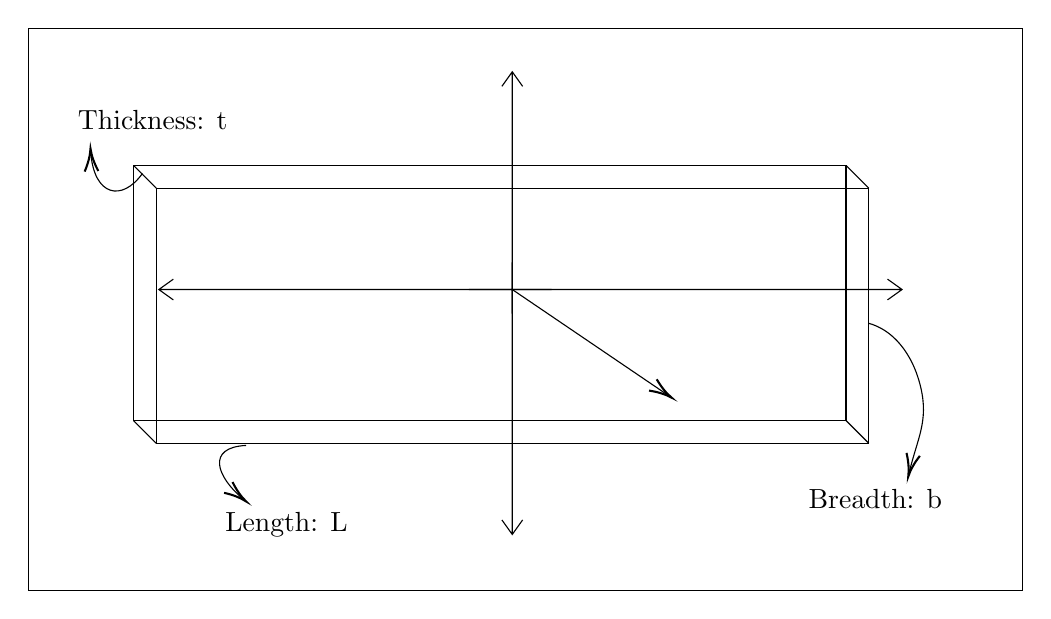
\begin{tikzpicture}[x=0.75pt,y=0.75pt,yscale=-1,xscale=1]

%uncomment if require: \path (0,380); %set diagram left start at 0, and has height of 380

%Shape: Rectangle [id:dp9376541203114244] 
\draw   (77.3,76.9) -- (556.3,76.9) -- (556.3,347.9) -- (77.3,347.9) -- cycle ;
%Shape: Rectangle [id:dp28813504467275786] 
\draw   (139,154) -- (482.3,154) -- (482.3,276.9) -- (139,276.9) -- cycle ;
%Shape: Rectangle [id:dp12139950976483205] 
\draw   (128,143) -- (471.3,143) -- (471.3,265.9) -- (128,265.9) -- cycle ;
%Straight Lines [id:da9780862958321793] 
\draw    (128,143) -- (139,154) ;
%Straight Lines [id:da8260715461726775] 
\draw    (128,265.9) -- (139,276.9) ;
%Straight Lines [id:da9959140145595331] 
\draw    (471.3,143) -- (482.3,154) ;
%Straight Lines [id:da8859058042690442] 
\draw    (471.3,265.9) -- (482.3,276.9) ;
%Shape: Axis 2D [id:dp43778346475831187] 
\draw  (289.65,202.79) -- (498.3,202.79)(310.51,97.9) -- (310.51,214.45) (491.3,197.79) -- (498.3,202.79) -- (491.3,207.79) (305.51,104.9) -- (310.51,97.9) -- (315.51,104.9)  ;
%Shape: Axis 2D [id:dp3306318563234224] 
\draw  (329.44,202.79) -- (140.22,202.79)(310.51,320.79) -- (310.51,189.68) (147.22,207.79) -- (140.22,202.79) -- (147.22,197.79) (315.51,313.79) -- (310.51,320.79) -- (305.51,313.79)  ;
%Straight Lines [id:da7916995417313895] 
\draw    (310.51,202.79) -- (385.65,253.78) ;
\draw [shift={(387.3,254.9)}, rotate = 214.16] [color={rgb, 255:red, 0; green, 0; blue, 0 }  ][line width=0.75]    (10.93,-3.29) .. controls (6.95,-1.4) and (3.31,-0.3) .. (0,0) .. controls (3.31,0.3) and (6.95,1.4) .. (10.93,3.29)   ;
%Curve Lines [id:da2860028750143563] 
\draw    (132.3,146.9) .. controls (122.55,160.55) and (109,158.04) .. (107.4,136.59) ;
\draw [shift={(107.3,134.9)}, rotate = 87.51] [color={rgb, 255:red, 0; green, 0; blue, 0 }  ][line width=0.75]    (10.93,-3.29) .. controls (6.95,-1.4) and (3.31,-0.3) .. (0,0) .. controls (3.31,0.3) and (6.95,1.4) .. (10.93,3.29)   ;
%Curve Lines [id:da8187064823260181] 
\draw    (182.3,277.9) .. controls (163,278.86) and (167.91,292.87) .. (180.86,303.73) ;
\draw [shift={(182.3,304.9)}, rotate = 218.16] [color={rgb, 255:red, 0; green, 0; blue, 0 }  ][line width=0.75]    (10.93,-3.29) .. controls (6.95,-1.4) and (3.31,-0.3) .. (0,0) .. controls (3.31,0.3) and (6.95,1.4) .. (10.93,3.29)   ;
%Curve Lines [id:da1294145311807896] 
\draw    (482,219) .. controls (493.3,221.9) and (503.3,232.9) .. (507.3,249.9) .. controls (511.16,266.3) and (505.71,274.33) .. (501.73,291.05) ;
\draw [shift={(501.3,292.9)}, rotate = 282.53] [color={rgb, 255:red, 0; green, 0; blue, 0 }  ][line width=0.75]    (10.93,-3.29) .. controls (6.95,-1.4) and (3.31,-0.3) .. (0,0) .. controls (3.31,0.3) and (6.95,1.4) .. (10.93,3.29)   ;

% Text Node
\draw (100,115) node [anchor=north west][inner sep=0.75pt]   [align=left] {Thickness: t};
% Text Node
\draw (171,309) node [anchor=north west][inner sep=0.75pt]   [align=left] {Length: L};
% Text Node
\draw (452,298) node [anchor=north west][inner sep=0.75pt]   [align=left] {Breadth: b};


\end{tikzpicture}\\
Fig : a cuboid to demonstrate the Dzhanibekov Effect.
\end{center}
Here the first and third principal axes are the Length axis ($\vb{I_3}$) and the depth axis ($\vb{I_1}$) respectively. The Intermediate axis is the breadth axis ($\vb{I_2}$). If we actually spin the cuboid around the breadth axis we will have unstable motion. 
\subsection{Proof}
We can refer to the diagram to actually see the effects and prove it for a random cuboid.
\begin{align*}
    \frac{d}{dt}\left(I_1\omega_1\right) &=  (I_2 - I_3)\omega_2\omega_3  \\
    \frac{d}{dt}\left(I_2\omega_2\right) &=  (I_3 - I_1)\omega_3\omega_1      \\
    \frac{d}{dt}\left(I_3\omega_3\right) &=  (I_1 - I_2)\omega_1\omega_2      \\
\end{align*}
If we see the moments of Inertia of the cuboid, we get $\vb{I_3}>\vb{I_2}>\vb{I_1}$
\subsubsection{Stability of the first }
Consider a rigid body rotating about its principal axes with moments of inertia $I_1$, $I_2$, and $I_3$. If the body is given a sudden twist about its intermediate axis $I_2$, then the resulting motion of the body can be described by the Euler equations:
\begin{align}
I_1 \dot{\omega}_1 &= (I_2 - I_3)\omega_2 \omega_3  \\
I_2 \dot{\omega}_2 &= (I_3 - I_1)\omega_3 \omega_1  \\
I_3 \dot{\omega}_3 &=  (I_1 - I_2)\omega_1 \omega_2  \\,
\end{align}
In the first case let us consider $\omega$ of the form:
\begin{align*}
    \va*{\omega} &= \omega_1 \hat{x} + \epsilon_2 \hat{y} + \epsilon_3 \hat{z}\\
    \textbf{We get after differentiating: }\\
    I_1 \ddot{\omega}_1 &= \frac{(I_2 - I_3)}{I_2}(I_3 - I_1)\omega_3^2 \omega_1 \\
    I_2 \ddot{\omega}_2 &= (I_3 - I_1)\omega_3 \omega_1  \\
    I_3 \ddot{\omega}_3 &=  (I_1 - I_2)\omega_1 \omega_2  \\,
\end{align*}

\newpage
\section{Sylvester's Law of inertia}
\section{Poinsot's Ellipsoid}
\newpage
\section{Dirac Delta in generalized coordinates}
The 3-D dirac delta function is not always the multiplication of the individual 1D dirac delta functions like in cartesian coordinate space $\ddelta = \delta(x)\delta(y)\delta(z)$.
\subsection{Generalized curvilinear coordinates}
Let the small displacement function be 
\begin{align*}
    d\vb{l} = h_1 de_1\hat{e_1} + h_2 de_2\hat{e_2} + h_3 de_3\hat{e_3}\\
\end{align*}
In the cartesian coordinates, $ \ddelta = \delta (y) \delta(x) \delta(z) $. In generalized coordinates, 
$\delta^3(\vb{r}) = \frac{\delta (e_1)}{h_1} \frac{\delta(e_2)}{h_2}  \frac{\delta(e_3)}{h_3}$
\begin{align*}
    h_i = \left[ \left( \dv{x}{e_i} \right)^2 + \left( \dv{y}{e_i} \right)^2 + \left( \dv{z}{e_i} \right)^2\right]^{1/2}
\end{align*}
\subsection{Spherical coordinates}
\begin{enumerate}
    \item [$e_1$] : r           [$h_1$] : 1    
    \item [$e_2$] : $\theta$    [$h_2$] : r
    \item [$e_3$] : $\phi$      [$h_3$] : r sin$\theta$
\end{enumerate}
\begin{align*}
    \delta^3(\vb{r}) = \frac{1}{r^2 sin\theta}\delta (r) \delta(\theta) \delta(\phi)
\end{align*}
Suppose that there is no azimuthal $\phi$ dependence, then we can take the $\phi$ part of the total integral out. We need the whole 3-D volume integral to be 1 over all space.
\begin{align*}
    \iiint_{\text{all space}} \delta^3(\vb{r}) \dd \tau &= \left( \iint \delta (r) \delta(\theta)\dd A' \right) \int^{2\pi}_0 \dd \phi \\
                                                         &= 2\pi \iint \delta (r) \delta(\theta)\dd A'    \\
    \text{Thus in the function the r and } \theta &\text{ parts go to 1 and the $\phi$ integral is left}\\
    \int^{2\pi}_{0} r^2 sin\theta \dd \phi &= 2\pi r^2 sin\theta \\
    \implies \delta^3(\vb{r}) &= \frac{1}{2\pi r^2 sin\theta}\delta (r) \delta(\theta)\\    
\end{align*}
Similarly, we can follow the similar method to arrive at the dirac delta function with no $ \theta or \phi$ dependence.
we get:
\begin{align*}
    \delta^3(\vb{r}-\vb{r_0}) &= \frac{1}{r^2 sin\theta}\delta (r-r_0) \delta(\theta-\theta_0) \delta(\phi-\phi_0)\\
                    &= \frac{1}{2 \pi r^2 sin\theta}\delta (r-r_0) \delta(\theta-\theta_0) \\
                    &= \frac{1}{4 \pi r^2} \delta (r-r_0)
\end{align*}
\subsection{Cylindrical coordinates}
\begin{enumerate}
    \item [$e_1$] : s           [$h_1$] : 1    
    \item [$e_2$] : $\phi$      [$h_2$] : s
    \item [$e_3$] : z           [$h_3$] : 1
\end{enumerate}
\begin{align*}
    \delta^3(\vb{s}-\vb{s_0}) &= \frac{1}{s}\delta (s-s_0) \delta(\phi-\phi_0) \delta(z-z_0)\\
                    &= \frac{1}{2 \pi s}\delta (s-s_0) \delta(z-z_0) \\
                    &= \frac{1}{2 \pi s} \delta (s-s_0)
\end{align*}
\newpage

\section{Standard Model}
\section{Ampere's Law on Finite Wires}
\section{Routhian Mechanics}
\newpage
\section{Routh's Rule}
\subsection{Stretch Rule}
This a rigorous proof that shows that if we keep the mass distribution about the axis same and the mass distribution is elongated along an axis parallel to the axis of rotation, then the moment of inertia is conserved.
\subsection{Statement}
\begin{example*}
    In classical mechanics, the stretch rule (sometimes referred to as Routh's rule) states that the moment of inertia of a rigid object is unchanged when the object is stretched parallel to an axis of rotation that is a principal axis, provided that the distribution of mass remains unchanged except in the direction parallel to the axis.
\end{example*}
\subsection{Proof}
Let the axis of rotation be the \va{z} axis.
\begin{align*}
    I_z &= \iiint_V \rho (x,y,z)r^2 dx dy dz\\
    &=\int^L_0dz\iint \rho(x,y,z)r^2 dx dy dz\\
\end{align*}
This can be written as the stretching is done along the $\vu{z}$ axis and thus we can take the $\dd{z}$ part of integral out. We can define the new Moment of Inertia is $I_{z'}$. We can change the length to $aL$ and thus the dz component changes to $z' = \frac{z}{a}$ and the mass distribution also changes to $\rho'(x',y',z') = \frac{\rho(x,y,z/a)}{a}$.
\begin{align*}
    I_{z'} &=\int^{aL}_0dz\iint \rho'(x',y',z')r^2 dx dy dz\\
    &= \int^{aL}_0dz\iint \rho'(x',y',z')r^2 dx dy dz\\
    &=\int^{L}_0adz'\iint \frac{\rho(x',y',\frac{z}{a})}{a}r^2 dx dy dz\\
    &=\int^{L}_0dz'\iint \rho(x,y,z')r^2 dx dy dz\\
    &=\iiint_V \rho (x,y,z')r^2 dx dy dz\\
    &=I_z
\end{align*}
This proves our statement and in turn the stretch rule.
\subsection{For some common Moments Of Inertia}
\begin{example*}
Routh's rule is a mnemonic formula for finding the moment of inertia of a symmetrical solid. The rule works for a circular or elliptical cylinder rotated about the cylinder axis, or for a circular or elliptical disk about any of the axes of symmetry. This is rarely used practically and just is used academically.
 \begin{align*}
     I = M\left(\frac{\text{sum of squares of semi-perpendicular axes}}{\text{3,4 or 5}}\right)
 \end{align*}
 \begin{enumerate}
     \item[3:] a rectangular lamina
     \item[4:] a elliptical lamina
     \item[5:] an ellipsoidal body. 
 \end{enumerate}
\end{example*}
\section{Calculus of Variations}
\section{Jacobian}
\section{Soliton}
\section{Kerr Effect}
\section{Pockels Effect}
\section{Komorebi}
\section{Legendre Transform}
\section{Legendre Polynomials}
\section{Rodrigues Formula}
\section{Hamiltonian Mechanics}
\section{Phase Space diagrams}


\end{document}

